\documentclass{ctexart}
\usepackage{graphicx}
\usepackage{amsmath}
\usepackage{geometry}
\usepackage[justification=centering]{caption}
\captionsetup{labelsep=space}
\usepackage[super]{cite}
\renewcommand\citeform[1]{[#1]}

\makeatletter
\renewcommand\@fnsymbol[1]{\ensuremath{\ifcase#1\or \dagger\or \ddagger\or \mathsection\or \mathparagraph\or \|\or **\or \dagger\dagger \or \ddagger\ddagger \else\@ctrerr\fi}}
\makeatother

\geometry{a4paper, left=2cm, right=2cm, top=2cm, bottom=2cm}
\setlength{\columnsep}{20pt}

\ctexset{
  section = {format=\raggedright\Large\bfseries},
  subsection = {format=\raggedright\large\bfseries}
}

\title{高压开关电源纹波对粒子辐射探测器系统噪声影响研究}

\author{
    罗宇琛 \quad 于向前\thanks{通信作者, E-mail: yuxiangqian@pku.edu.cn; Corresponding author, E-mail: yuxiangqian@pku.edu.cn} \quad 王玲华 \quad 陈鸿飞 \quad 施伟红 \\ 王永福 \quad 王游龙 \quad 杨芯 \quad 宗秋刚 \quad 邹鸿 \\[0.5ex]
    \small{(北京大学 地球与空间科学学院,北京,100871)}
}

\date{}

\begin{document}

\maketitle
\thispagestyle{empty}
\begin{quote}
    \noindent\textbf{摘要} \quad 粒子辐射探测器需要在高压开关电源的偏置下才能正常工作,高压开关电源的纹波直接影响粒子辐射探测器系统的噪声。本文首先通过理论分析,建立噪声传递函数,得到了从高压开关电源纹波到粒子辐射探测器系统输出噪声的定量理论模型,并进行了系统仿真验证。仿真结果与理论结果相吻合,验证了理论的适用性。本文的研究可以为后续粒子辐射探测器高压开关电源的研制提供参考。
    \vspace{0em}
    
    \noindent\textbf{关键词} \quad 粒子辐射探测器;高压电源;电压纹波;噪声分析
\end{quote}

\vspace{0em}

\begin{center}
    \large\bfseries Research on the Impact of High-Voltage Bias Switch Mode Power Supply Ripple on Noise in Particle Radiation Detection Systems
\end{center}
\vspace{0em}

\begin{center}
    Yuchen Luo, \quad Xiangqian Yu\footnotemark[1], \quad Linghua Wang, \quad Hongfei Chen, \quad Weihong Shi, \\
    Yongfu Wang, \quad Youlong Wang, \quad Xinxin Yang, \quad Qiugang Zong, \quad Hong Zou \\[0.5ex]
    \small{(School of Earth and Space Sciences, Peking University, Beijing, 100871)}
\end{center}
\vspace{0em}

\begin{quote}
    \noindent\textbf{Abstract} \quad [Background] Output ripple from high-voltage switching power supplies degrades the energy resolution of particle detectors, but a quantitative model of this noise source is lacking. [Purpose] This study develops and validates a quantitative model linking power supply ripple to the output noise in a Si-PIN detector system. [Methods] A noise transfer function for the full signal chain was established and validated against a PySpice system simulation, with noise quantified by the energy spectrum's FWHM. [Results] The simulation shows strong agreement with the model at high frequencies (>10 kHz), with <5\% deviation. A 2V peak-to-peak ripple at 70 kHz introduces ~1 keV FWHM of noise. [Conclusions] This work provides a validated quantitative framework confirming ripple as a major noise contributor and offers an essential tool for designing low-noise high-voltage power supplies.
    \vspace{0em}
    
    \noindent\textbf{Keywords} \quad Semiconductor detectors; High-voltage bias power supply; Voltage ripple; Noise analysis
\end{quote}

\twocolumn

\section{引言}

粒子辐射探测在空间物理、高能粒子物理及医学成像等领域至关重要\cite{1, 2, 3}。粒子辐射探测器依赖高压开关电源,以扩大耗
尽区并在耗尽区内形成强电场,驱动电离产生的电荷载流子(电子-空穴/离子对)向电极迁移,生成可测电信号。

高压开关电源纹波通过各种耦合机制影响探测器输出,增加噪声,降低信噪比,并导致数据失真\cite{4}。低纹波的高压开关电源可以确保探测器耗尽区电场的时间一致性,使载流子的漂移稳定;同时减少耦合到输出端的噪声,提高信噪比及能量分辨率\cite{5}。以前人们对高压开关电源纹波对粒子辐射探测器系统噪声的影响的研究定性居多,缺少定量研究\cite{6, 7}。本文将从Si-PIN 型粒子辐射探测器电路结构出发,建立从高压开关电源纹波到探测器系统输出噪声的定量理论模型,并通过系统仿真验证其适用性,为提升粒子辐射探测器的测量精度提供理论参考。


\section{理论分析}

\subsection{电路分析}

对于 Si-PIN 型粒子辐射探测器系统,与高压开关电源纹波相关的电路可以大致分为电源滤波电路、电荷敏感前置放大器和整形放大电路三部分,如图\ref{fig:overall_system}所示。

\begin{figure}[!h]
    \centering
    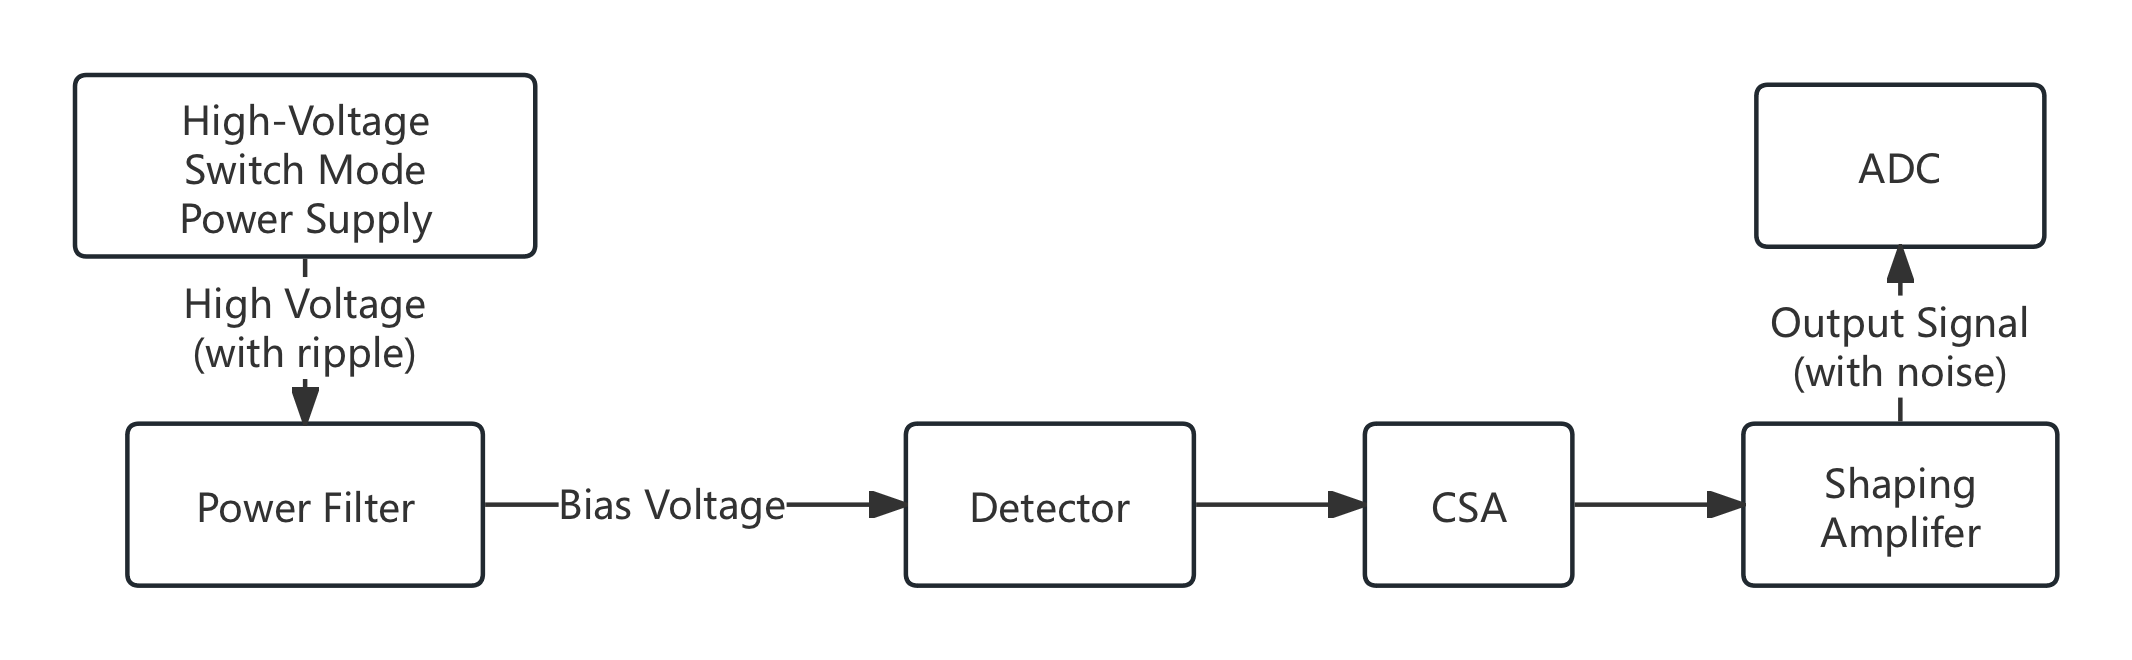
\includegraphics[width=\linewidth]{./overall_system.png}
    \caption{高压电源纹波在探测器系统中的耦合路径示意图 \\ Fig. 1 Schematic of the coupling path of high-voltage power supply ripple in the detector system}
    \label{fig:overall_system}
\end{figure}

图\ref{fig:power_filter}所示为电源滤波电路的等效电路,可以看作由两个RC 低通滤波器级联而成的二阶滤波架构,用于抑制高频噪声\cite{8}。高压开关电源由BBV输入,经过该滤波网络后,通过H1端子为探测器提供偏置电压。

\begin{figure}[!h]
    \centering
    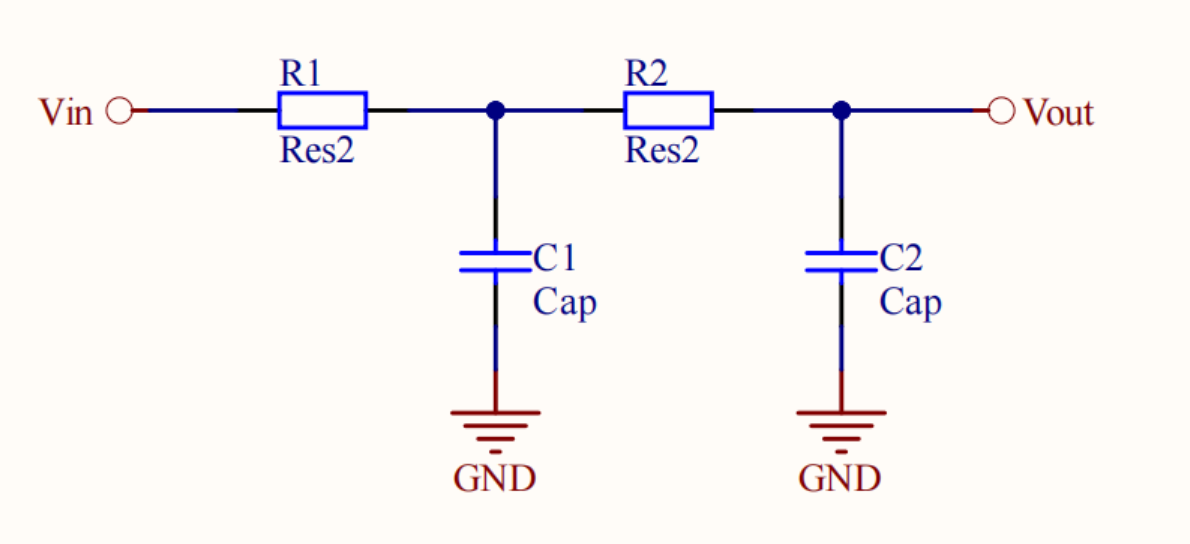
\includegraphics[width=\linewidth]{./power_filter.png}
    \caption{高压偏置电源滤波网络电路图 \\ Fig. 2 Circuit diagram of the high-voltage bias power supply filter network}
    \label{fig:power_filter}
\end{figure}

图\ref{fig:detector_csa}所示为探测器与电荷敏感前置放大器的结构,探测器可以等效为一个二极管和结电容 $C_{\mathrm{d}}$ 并联。在完全耗尽的情况下,结电容 $C_{\mathrm{d}}$ 可由下式计算\cite{9}:
\begin{equation*}
C_{\mathrm{d}} = \frac{\varepsilon_0 \varepsilon_{\mathrm{r}} S}{D_{\mathrm{d}}}
\end{equation*}
其中 $A_{\mathrm{s}}$ 为探测器的等效正对面积(通常在 mm² 量级),$D_{\mathrm{d}}$ 为探测器厚度(通常在 um 量级)。由此可计算得 $C_{\mathrm{d}}$ 通常在 pF 量级。

\begin{figure}[!h]
    \centering
    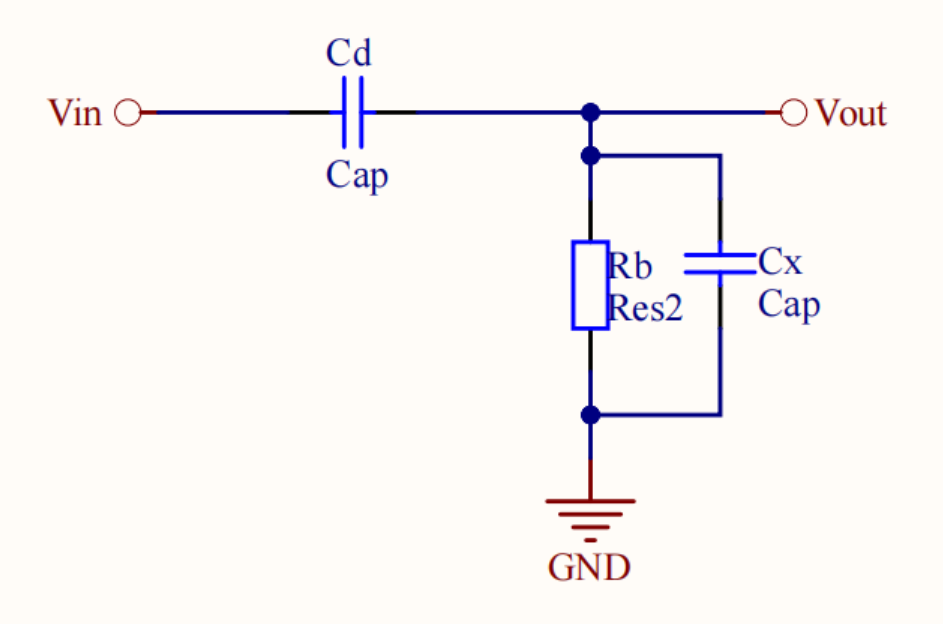
\includegraphics[width=\linewidth]{./detector.png}
    \caption{Si-PIN探测器与电荷敏感前置放大器电路图 \\ Fig. 3 Circuit diagram of the Si-PIN detector and charge-sensitive preamplifier (CSA)}
    \label{fig:detector_csa}
\end{figure}

偏置电压 $V_{\mathrm{bias}}$ 的大小与探测器的厚度有关。耗尽层厚度 d 与偏置电压的关系为 $d = \sqrt{2\varepsilon_0\varepsilon_{\mathrm{r}}\mu V_{\mathrm{bias}} / \rho}$ \cite{9},为了使探测器完全耗尽,偏置电压至少应该满足
\begin{equation*}
D_{\mathrm{d}} = \sqrt{\frac{2\varepsilon_0\varepsilon_{\mathrm{r}}\mu V_{\mathrm{bias}}}{\rho}}
\end{equation*}
即
\begin{equation*}
V_{\mathrm{bias}} = \frac{D_{\mathrm{d}}^2\rho}{2\varepsilon_0\varepsilon_{\mathrm{r}}\mu}
\end{equation*}
其中 $\rho$ 为电阻率,$\mu$ 为多数载流子迁移率。取 $\varepsilon = \varepsilon_0 = 8.85 \times 10^{-12} \text{ F/m}$, $\rho = 10 \text{k}\Omega \cdot \text{cm}$,$\mu = 1200 \text{ cm}^2/(\text{V} \cdot \text{s})$,可计算得对于厚度为 $D_{\mathrm{d}} = 200\,\mu\text{m}$ 的探测器,需要 $V_{\mathrm{bias}} \approx 200 \text{ V}$。

$C_{\mathrm{x}}$为隔直电容,其容值通常在nF到$\mu$F量级,用于阻隔来自探测器的直流电流。探测器产生的电荷信号经$C_{\mathrm{x}}$耦合至电荷敏感放大器(CSA),经由CSA被放大至适合后续数字信号处理的电平。

整形放大电路通常与数模转换器一起内置在ASIC中,将放大后的信号整形为类高斯波形,为后续的模数转换做准备。本文假定该电路采用CR-RC滤波器的架构\cite{10},具有成形时间$\tau$,同时提供增益$A_0$。

\subsection{纹波模型}

如图\ref{fig:ripple}所示,高压开关电源的纹波通常表现为周期性的锯齿波,主要由开关器件的 PWM 控制所引起\cite{11},其波形的上升沿和下降沿的斜率取决于开关频率、占空比以及控制策略,并直接决定了纹波幅度及其频谱分布\cite{12}。

\begin{figure}[!h]
    \centering
    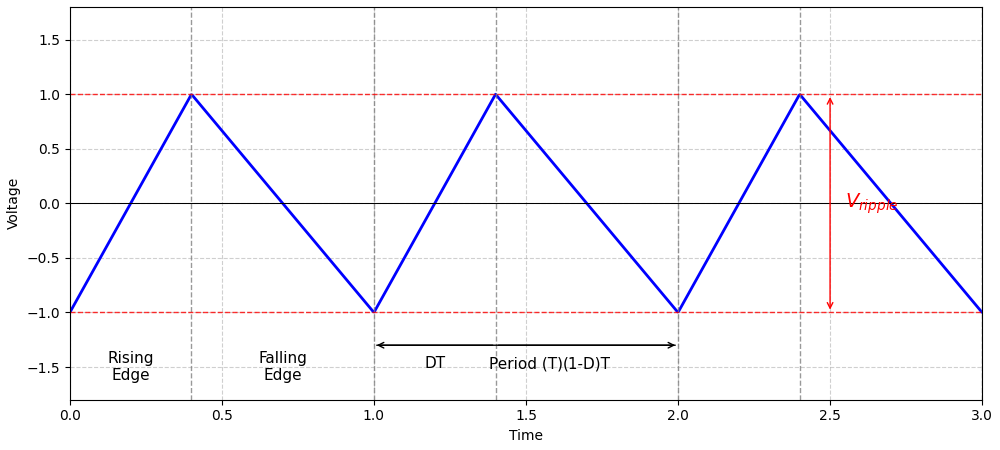
\includegraphics[width=\linewidth]{./ripple.png}
    \caption{典型高压开关电源输出纹波波形示意图 \\ Fig. 4 Typical output ripple waveform of a high-voltage switching mode power supply}
    \label{fig:ripple}
\end{figure}

为便于分析,将纹波波形等效为频率、功率相同的正弦波。纹波波形近似为锯齿波,其电压随时间线性变化。对于峰峰值为 $V_{\mathrm{ripple}}$、周期为 $T$ 的锯齿波,其电压可表示为 $v(t) = \frac{V_{\mathrm{ripple}}}{T}t - \frac{V_{\mathrm{ripple}}}{2}$(其中 $t \in [0, T]$)。该波形的归一化平均功率(即均方电压 $V_{\mathrm{rms}}^2$)为
\begin{align*}
P_{\mathrm{ripple}} &= V_{\mathrm{rms,ripple}}^2 = \frac{1}{T}\int_0^T v(t)^2 dt \\
&= \frac{1}{T}\int_0^T \left(\frac{V_{\mathrm{ripple}}}{T}t - \frac{V_{\mathrm{ripple}}}{2}\right)^2 dt = \frac{V_{\mathrm{ripple}}^2}{12}
\end{align*}
对于峰峰值为 $V_{\mathrm{pp,sin}}$ 的正弦波,其振幅为 $V_{\mathrm{pp,sin}}/2$,其归一化平均功率为
\begin{equation*}
P_{\mathrm{sin}} = V_{\mathrm{rms,sin}}^2 = \left(\frac{V_{\mathrm{pp,sin}}/2}{\sqrt{2}}\right)^2 = \frac{V_{\mathrm{pp,sin}}^2}{8}
\end{equation*}
令二者的平均功率相等,即 $P_{\mathrm{ripple}} = P_{\mathrm{sin}}$,得
\begin{equation*}
\frac{V_{\mathrm{ripple}}^2}{12} = \frac{V_{\mathrm{pp,sin}}^2}{8}
\end{equation*}
解出等效正弦波的峰峰值 $V_{\mathrm{pp,sin}}$为
\begin{equation*}
V_{\mathrm{pp,sin}} = \sqrt{\frac{8}{12}}V_{\mathrm{ripple}} = \sqrt{\frac{2}{3}}V_{\mathrm{ripple}}
\end{equation*}
因此,在后续分析中,将峰峰值为 $V_{\mathrm{ripple}}$ 的纹波等效为峰峰值为 $\sqrt{\frac{2}{3}}V_{\mathrm{ripple}}$ 的正弦波。

\subsection{纹波耦合}

为定量计算高压开关电源纹波对探测器系统输出噪声的影响,需基于线性电路理论,分析其通过后续电路中频率响应\cite{13}。具体方法为:首先建立纹波传播路径的传递函数模型,再将其与纹波电压频谱相乘,即可得到输出端信号的特征。
电源电压从电源滤波电路的输入端接入,可将其等效为叠加于直流高压上的小幅值正弦交流电压源,并设其幅值为 $v_{\mathrm{ripple}}$,频率为 $f_{\mathrm{ripple}}$。
电源滤波电路可建模为两个 RC 滤波器级的级联。电源滤波电路的传递函数为
\begin{equation}
H_\text{powerFilter}(f) = \frac{1}{1 + j2\pi f R_1 C_1} \cdot \frac{1}{1 + j2\pi f R_2 C_2}
\end{equation}
接下来分析偏置电压纹波耦合至 CSA 输出端的频率响应。在 $V_{\mathrm{bias}}$ 处叠加频率为 $f$ 的小幅值交流电压源 $u$,考虑到运算放大器的理想特性,其反相输入端为虚地,故认为该点电势为0。可求得探测器阳极电压$u_1$为
\begin{equation}
u_1 = u \cdot \frac{j2\pi f C_{\mathrm{d}} R_{\mathrm{b}}}{1 + j2\pi f C_{\mathrm{d}} R_{\mathrm{b}} + j2\pi f C_{\mathrm{d}} R_{\mathrm{b}}}
\end{equation}
CSA 的输出电压 $u_2$ 与探测器阴极电压 $u_{\mathrm{d}}$ 的增益由反馈网络阻抗 $Z_{\mathrm{f}}$ 与输入支路阻抗 $Z_{\mathrm{s}}$ 的阻抗比决定,即
\begin{equation}
\frac{u_2}{u_1} = -\frac{Z_{\mathrm{f}}}{Z_{\mathrm{s}}} = - \frac{1 / (j2\pi f C_{\mathrm{f}})}{R_{\mathrm{s}} + 1/(j2\pi f C_{\mathrm{f}})}
\end{equation}
联立式(5)(6),可得输出电压 $u_2$ 的表达式为
\begin{equation}
u_2 = - \frac{j2\pi f C_{\mathrm{d}} R_{\mathrm{b}}}{(1 + 2j\pi f C_{\mathrm{d}} R_{\mathrm{b}})(1 + j2\pi f C_{\mathrm{f}}R_{\mathrm{s}})}
\end{equation}
从而,从探测器偏置端到 CSA 输出端的纹波耦合传递函数为
\begin{equation}
H_\text{csa}(f) = \frac{u_2}{u} = - \frac{j2\pi f C_{\mathrm{d}} R_{\mathrm{b}}}{(1 + 2j\pi f C_{\mathrm{d}} R_{\mathrm{b}})(1 + j2\pi f C_{\mathrm{f}}R_{\mathrm{s}})}
\end{equation}
接下来计算整形放大电路的响应。假设整形电路的波形成形时间为$\tau$,增益为$A_0$,可计算其传递函数为
\begin{equation}
H_\text{shaper}(f) = A_0 \frac{j2\pi f \tau}{(1 + j2\pi f \tau)^2}
\end{equation}
综合考虑各级电路的频率响应,最终输出的纹波幅值为
\begin{multline}
v_{\mathrm{ripple,out}} = \\
 v_{\mathrm{ripple,in}} |H_\text{powerFilter}(f)|^2 |H_\text{csa}(f)|^2 |H_\text{shaper}(f)|^2
\end{multline}
换算成以 eV 为单位的半峰全宽(Full Width at Half Maximum, FWHM)\cite{14}得
\begin{equation}
\mathrm{FWHM} = 2.35\times3.62\times \frac{\mathrm{ENC}}{q} = 8.5 \cdot \frac{e\cdot v_{\mathrm{ripple,out}} \cdot C_{\mathrm{f}}}{A_0q}
\end{equation}
其中 $e$ 为自然常数,$C_{\mathrm{f}}$ 为反馈电容值,$q$ 为元电荷量。


\section{仿真}

为验证前述理论模型的准确性,本文搭建了一个基于Spice和Python的探测器仿真系统,实现了模拟粒子射入到ADC计数的过程,通过测量纹波对计数结果的影响,定量评估高压开关电源纹波对探测器输出噪声的影响。

\subsection{仿真算法}

本文基于 PySpice 框架搭建了如图\ref{fig:circ_sim}所示的探测器系统Spice仿真电路,包含了电源滤波电路、PIN光电二极管等效电路、电荷敏感放大器及整形放大电路。小幅值正弦交流电压源V1模拟高压开关电源纹波,脉冲电流源Id模拟粒子射入产生的电流。

\begin{figure}[!h]
    \centering
    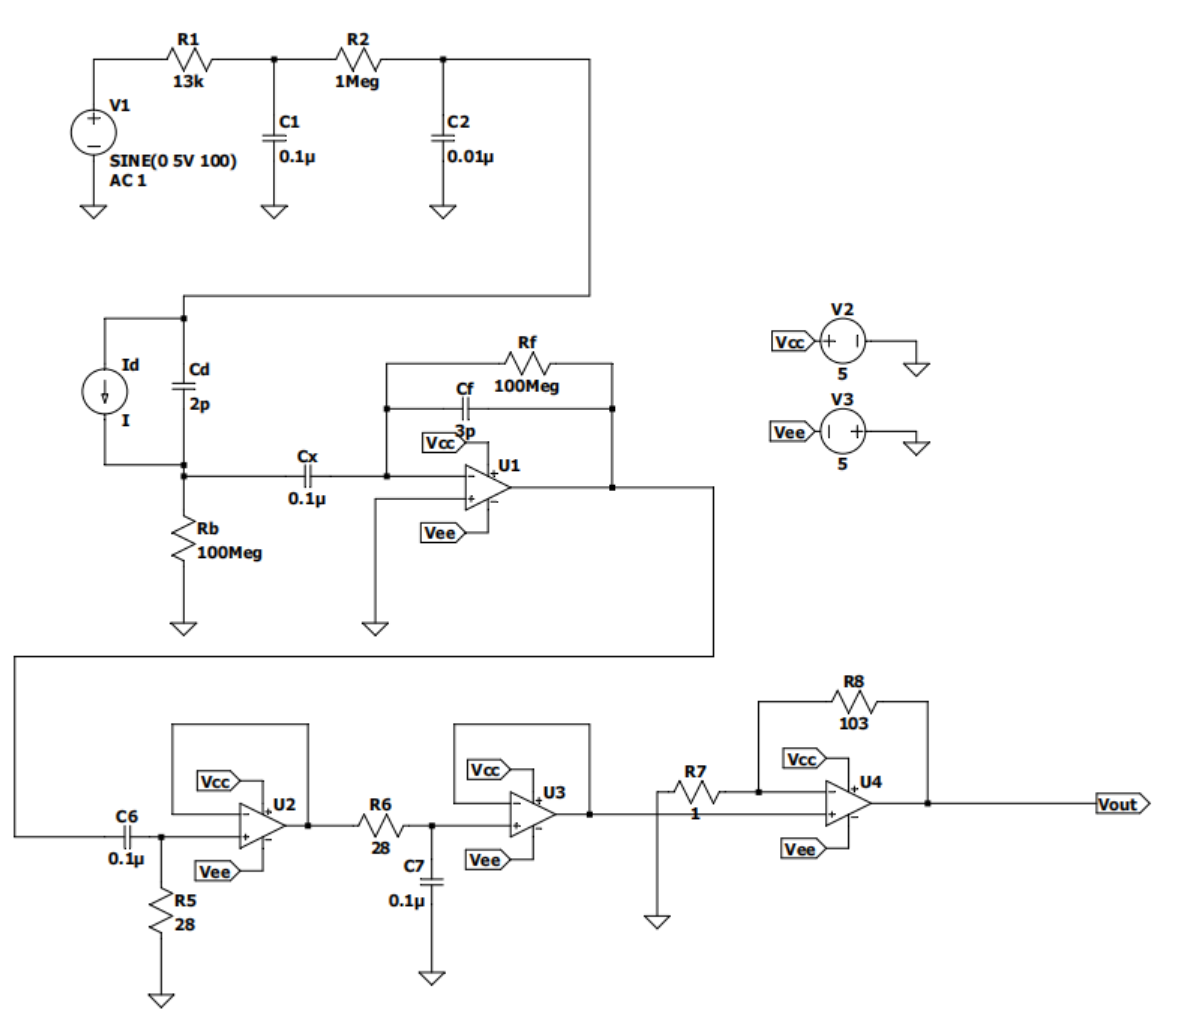
\includegraphics[width=\linewidth]{./circ_sim.png}
    \caption{用于纹波噪声分析的探测器系统SPICE仿真电路 \\ Fig. 5 SPICE simulation circuit of the detector system for ripple noise analysis}
    \label{fig:circ_sim}
\end{figure}

根据探测器收到的粒子能量,仿真将Id设置为幅值$0.4\,\mu\mathrm{A}$、脉冲宽度$1\,\mu\mathrm{s}$、周期$0.987\mathrm{ms}$(频率约为$1013\mathrm{Hz}$)的脉冲电流,用以模拟$9.05\mathrm{MeV}$的粒子以每秒约1000个的通量射入探测器。系统对该电流脉冲的响应为在输出端Vout产生一个类高斯形的电压脉冲(如图\ref{fig:circ_sim_response}所示),脉冲高度与粒子能量成正比。

\begin{figure}[!h]
    \centering
    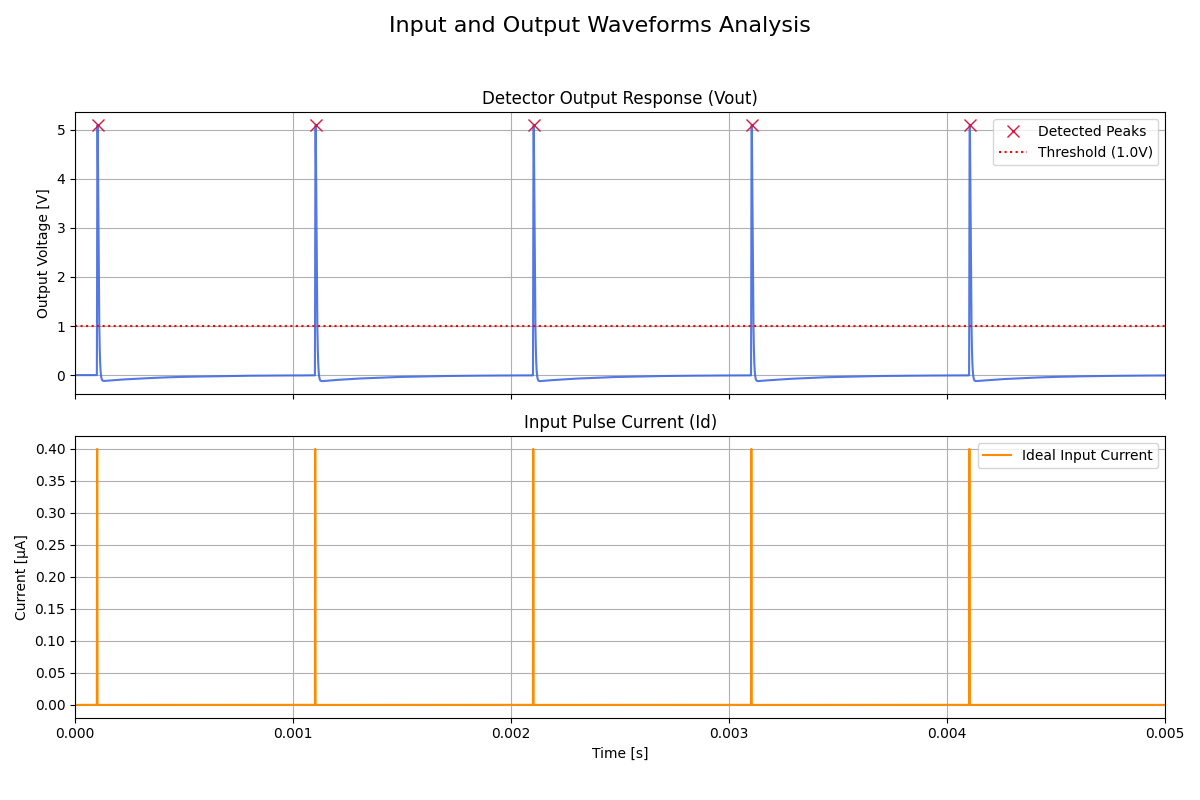
\includegraphics[width=\linewidth]{./circ_sim_response.png}
    \caption{探测器系统对单个粒子入射的输出电压脉冲响应 \\ Fig. 6 Output voltage pulse response of the detector system to a single particle event}
    \label{fig:circ_sim_response}
\end{figure}

为模拟真实探测器的信号处理过程,本文对瞬态仿真输出波形进行分析,设置阈值(1.0V)来识别并测量每个输出脉冲的峰高,并将收集到的所有脉冲峰高数据构建成能谱。电源纹波会导致输出脉冲的基线波动,从而使能谱的峰位展宽。本文以能谱峰的FWHM作为关键指标,定量评估不同参数的纹波对探测器能量分辨率的影响。为更准确地反映真实探测器性能,本文在仿真中引入了额外的高斯噪声,以模拟电子学噪声等系统固有噪声源。此外,由于电源纹波并非高斯白噪声,导致的能谱展宽具有非高斯特性,直接计算FWHM存在困难,叠加高斯噪声可使展宽峰形近似于高斯分布,便于计算FWHM。关于纹波非高斯性的详细讨论见3.3节。图\ref{fig:circ_sim_fwhm}为纹波幅值$3.0\mathrm{V}$,纹波频率$10\mathrm{kHz}$,固有噪声$5.00\mathrm{keV}$的能谱结果,测得总噪声FWHM为$6.98\mathrm{keV}$,即纹波引入的噪声为$\sqrt{6.98^2-5.00^2}\mathrm{keV}\approx4.87\mathrm{keV}$。

\begin{figure}[!h]
    \centering
    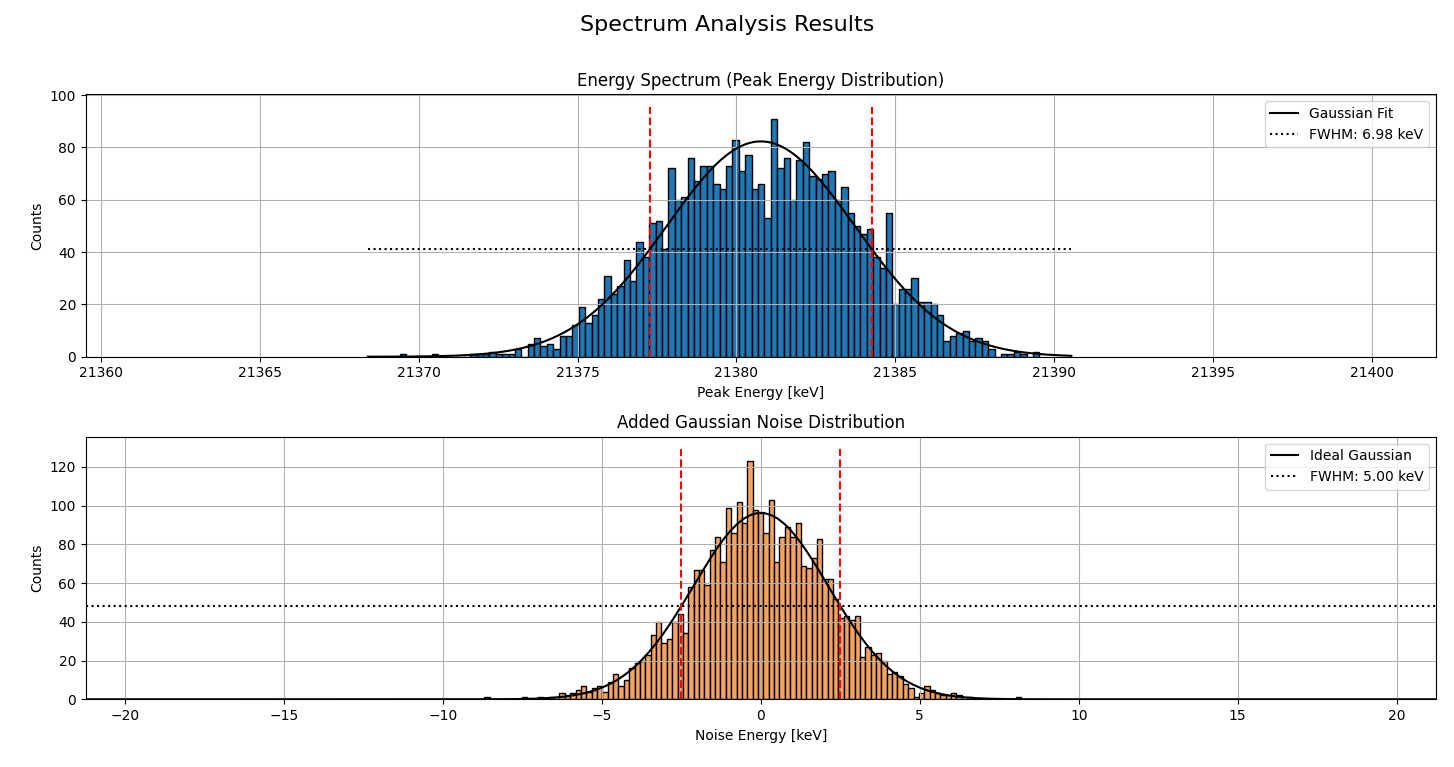
\includegraphics[width=\linewidth]{./circ_sim_fwhm.png}
    \caption{仿真得到的探测器输出信号能谱及FWHM计算示例 \\ Fig. 7 Example of the simulated detector output energy spectrum and FWHM calculation}
    \label{fig:circ_sim_fwhm}
\end{figure}

仿真使用的电路元件参数见表\ref{tab:params}。

\begin{table}[!h]
    \centering
    \caption{仿真电路元件参数 \\ Table 1 Parameters of the simulation circuit components}
    \label{tab:params}
    \begin{tabular}{lll}
        \hline
        变量名 & 值 & 描述 \\
        \hline
        $t$ & $2.8\,\mu\mathrm{s}$ & 整形放大电路的时间常数 \\
        $R_1$ & $13 \mathrm{k\Omega}$ & 电源滤波电路电阻 \\
        $C_1$ & $0.1\,\mu\mathrm{F}$ & 电源滤波电路电容 \\
        $R_2$ & $10 \mathrm{M\Omega}$ & 电源滤波电路电阻 \\
        $C_2$ & $0.01\,\mu\mathrm{F}$ & 电源滤波电路电容 \\
        $C_{\mathrm{d}}$ & $2\text{pF}$ & 探测器结电容 \\
        $C_{\mathrm{x}}$ & $0.1\,\mu\mathrm{F}$ & 隔直电容 \\
        $C_{\mathrm{f}}$ & $3 \mathrm{pF}$ & 反馈电容 \\
        $R_{\mathrm{b}}$ & $100 \mathrm{M\Omega}$ & 偏置电阻 \\
        $R_{\mathrm{f}}$ & $200 \mathrm{M\Omega}$ & 反馈电阻 \\
        $A_0$ & $38 \times e$ & 整形放大电路的增益 \\
        \hline
    \end{tabular}
\end{table}

\subsection{仿真结果}

本文分别对纹波幅值$1.0\mathrm{V}$至$10.0\mathrm{V}$,纹波频率$100\mathrm{Hz}$至$100\mathrm{kHz}$的纹波对探测器输出Vout的影响进行了仿真,每个数据点仿真3秒(约3000个峰值),并将仿真结果与理论计算结果进行比较,如图\ref{fig:circ_sim_result}所示。虽然仿真结果在低频段($<10\mathrm{kHz}$)显著小于理论结果,但在高频段($>10\mathrm{kHz}$)与理论结果基本吻合,最高误差不超过5\%。对于高压开关电源纹波的典型频率(60~300kHz)\cite{15},本文得出的模型适用性良好。在70kHz的典型开关频率下,峰峰值为2V(即幅值为1V)的纹波在探测器系统输出端引入约1 keV FWHM的噪声,显著降低系统能量分辨率。

\begin{figure}[!h]
    \centering
    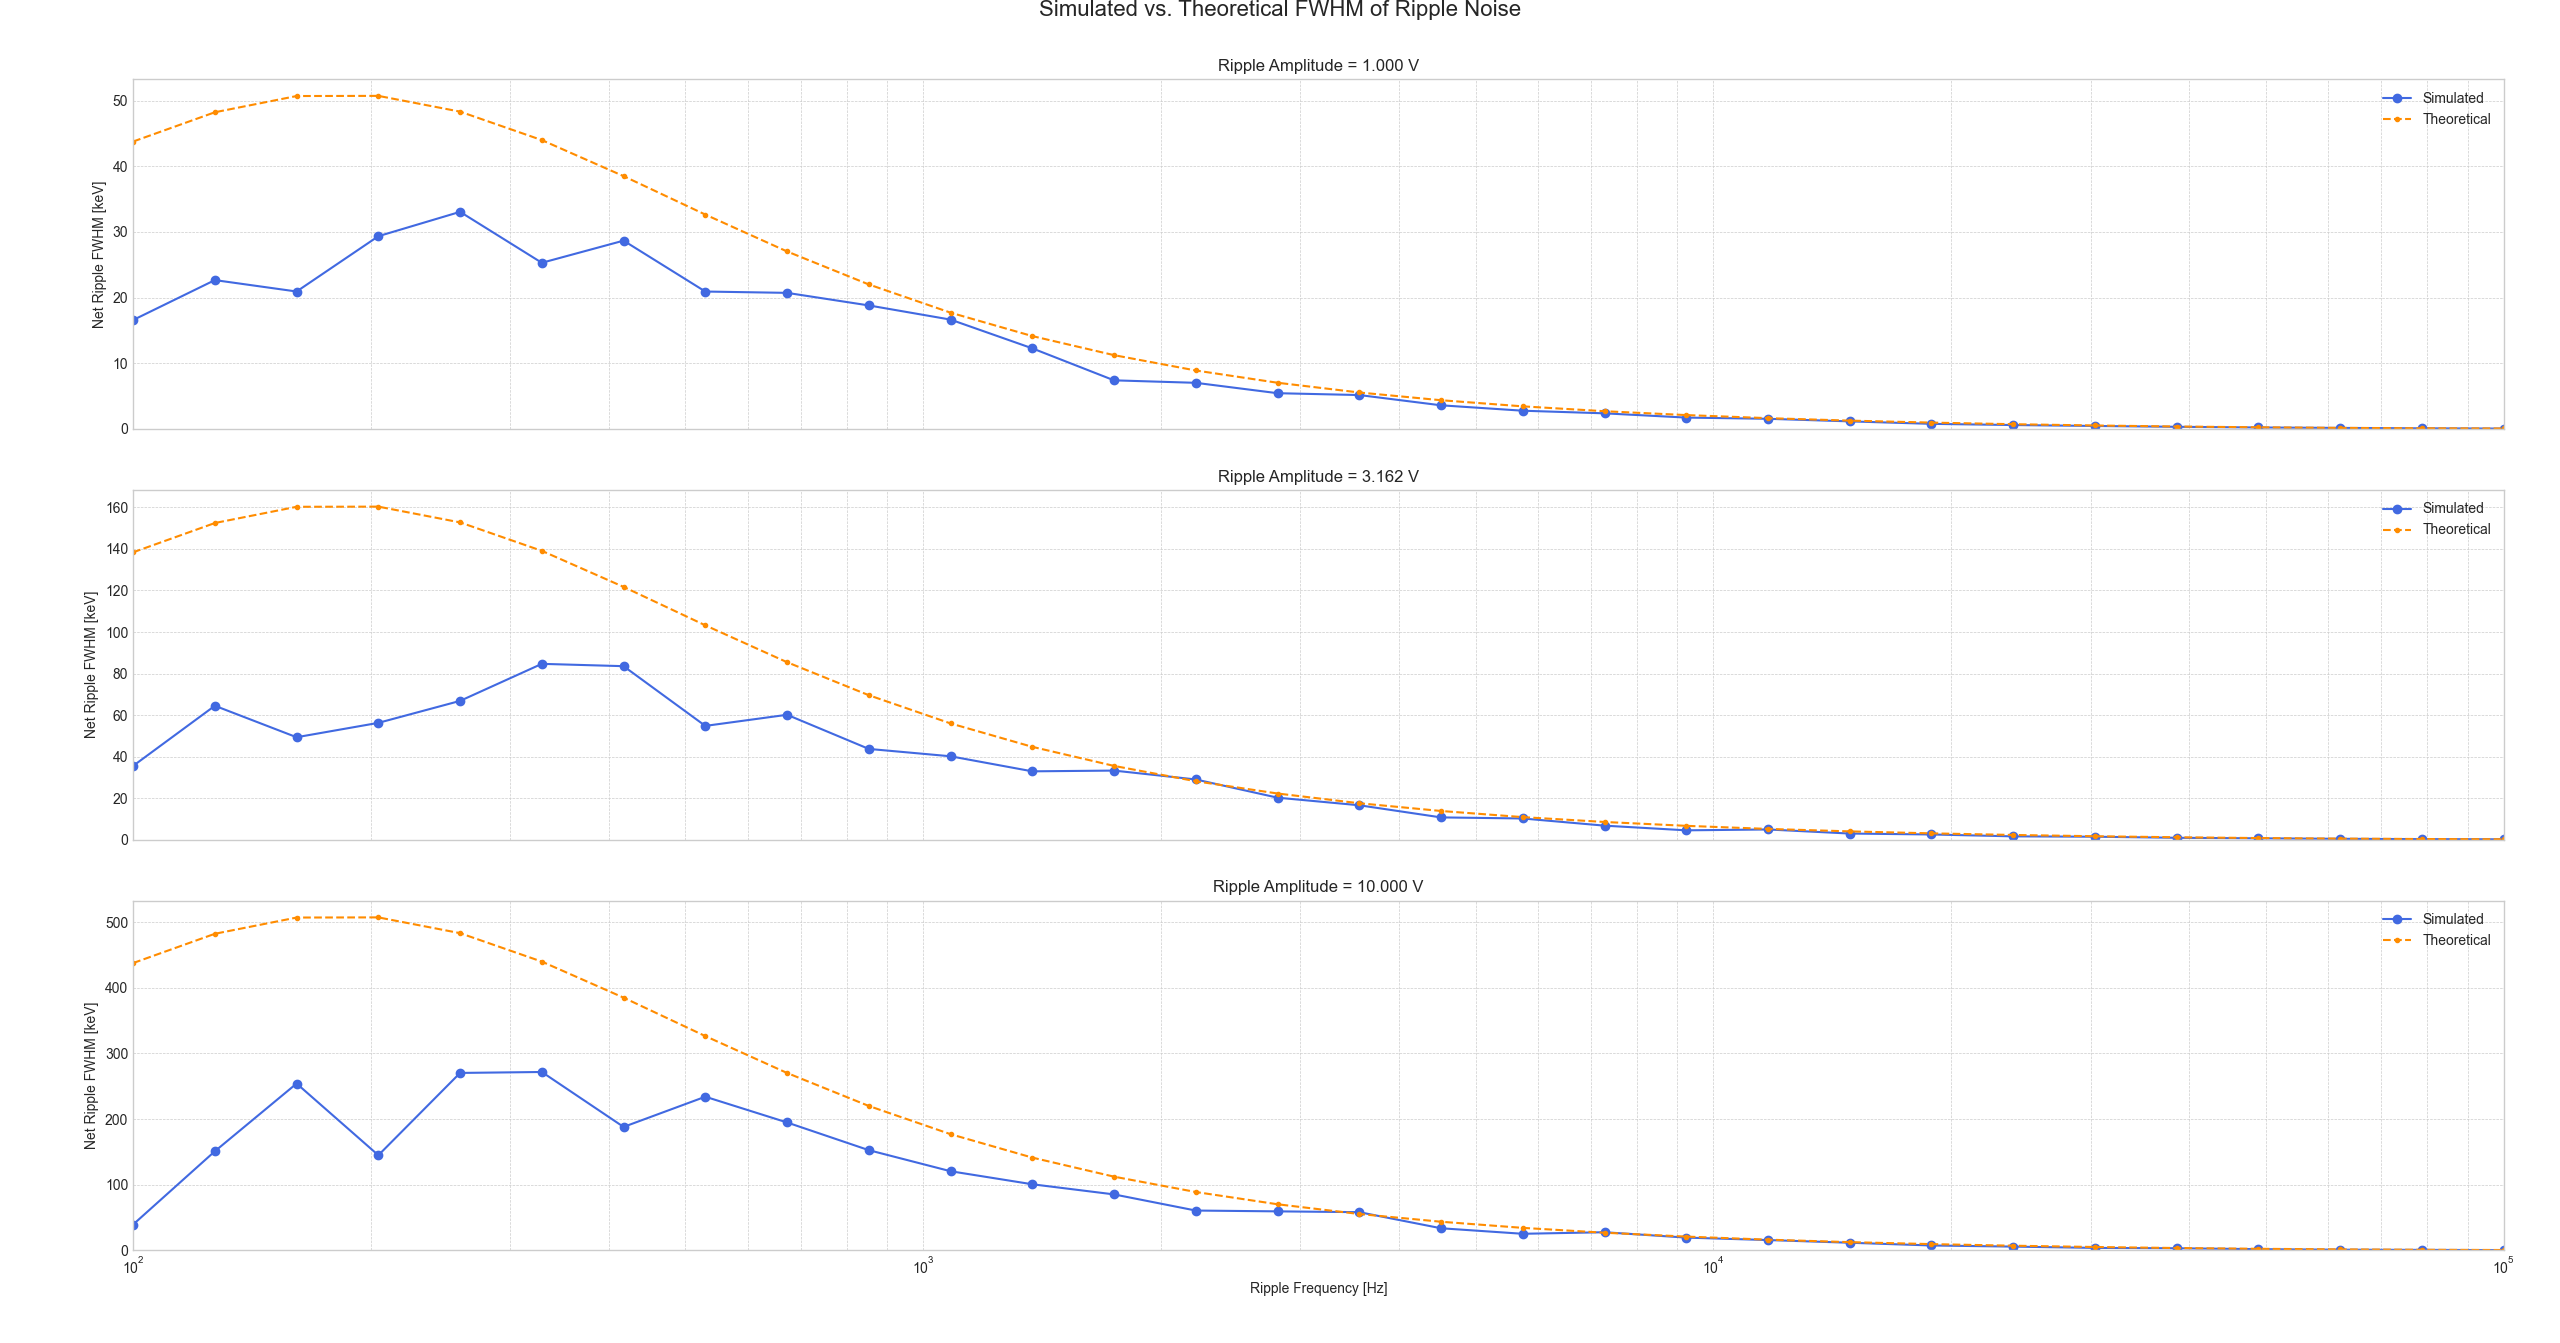
\includegraphics[width=\linewidth]{./circ_sim_result.png}
    \caption{高压电源纹波对探测器系统输出噪声的影响(仿真结果与理论结果对比) \\ Fig. 8 Impact of high-voltage power supply ripple on detector system output noise (comparison between simulation and theoretical results)}
    \label{fig:circ_sim_result}
\end{figure}

\subsection{纹波非高斯性影响分析}

在噪声分析中,通常将噪声源视为高斯白噪声\cite{13},其耦合到探测器输出端形成高斯形的能峰,可由FWHM衡量。但高压开关电源纹波通常包含确定的周期性分量(锯齿波或方波),并非高斯白噪声,其耦合到探测器输出端通常成为基频谐波,无法直接用FWHM衡量。

设纹波耦合到探测器输出端的功率为$v_\text{ripple}^2$,假设成为正弦波,则幅值分布为
\begin{equation*}
P_\text{sine}(x)=\frac{1}{\pi\sqrt{2v_\text{ripple}^2-x^2}}
\end{equation*}
假设为高斯白噪声,则幅值分布为
\begin{equation*}
P_\text{gaussian}(x)=G(0, v_\text{ripple}^2)
\end{equation*}
设输出端固有噪声功率为$v_\text{other}^2$,两种假设下幅值分布分别为
\begin{equation*}
P_\text{total,sine}(x)=P_\text{sine}(x)*G(0, v_\text{other}^2)
\end{equation*}
和
\begin{equation*}
P_\text{total,gaussian}(x)=G(0, v_\text{other}^2+v_\text{ripple}^2)
\end{equation*}
图\ref{fig:non_gausian_effect}、图\ref{fig:non_gausian_effect_num}展示了在两种假设下,在探测器输出端存在不同功率固有噪声时,纹波耦合到探测器输出端的幅值分布以及总FWHM差异。当固有噪声的功率超过纹波噪声两倍时,两种假设下的FWHM差异在5\%以内,可以认为纹波非高斯性引入的误差是可接受的;当固有噪声的功率低于纹波噪声两倍时,两种假设下的FWHM差异最高可达约31\%,需要考虑纹波非高斯性引入的误差。

\begin{figure}[!h]
    \centering
    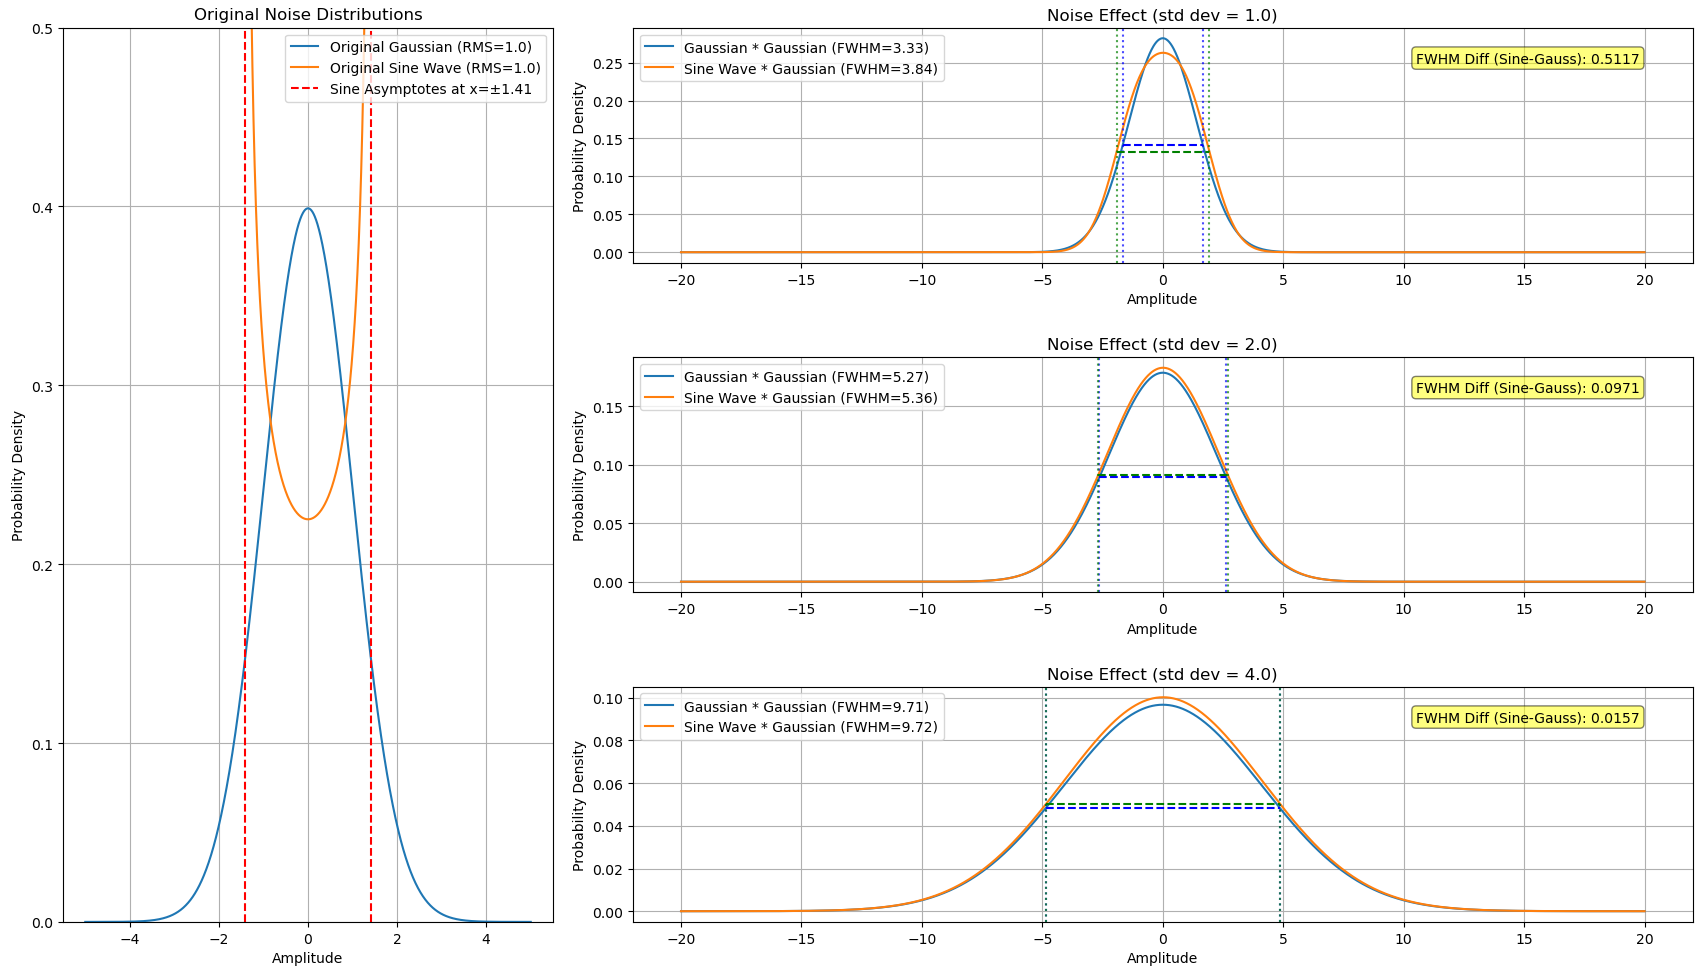
\includegraphics[width=\linewidth]{./non_gausian_effect.png}
    \caption{正弦噪声与高斯噪声假设下输出信号的幅值分布对比 \\ Fig. 9 Comparison of output signal amplitude distributions under sinusoidal and Gaussian noise assumptions}
    \label{fig:non_gausian_effect}
\end{figure}

\begin{figure}[!h]
    \centering
    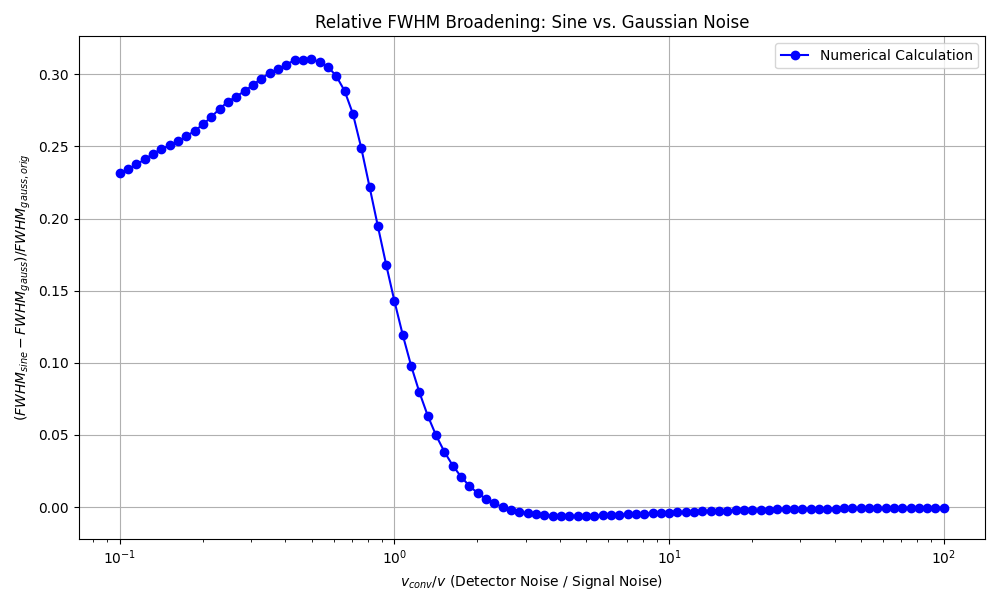
\includegraphics[width=\linewidth]{./non_gausian_effect_num.png}
    \caption{不同固有噪声水平下纹波噪声非高斯性对FWHM计算的影响 \\ Fig. 10 Impact of ripple noise non-Gaussianity on FWHM calculation at different intrinsic noise levels}
    \label{fig:non_gausian_effect_num}
\end{figure}


\section{总结}

本文对高压开关电源纹波在Si-PIN型粒子辐射探测器中引入的噪声进行了定量的分析,建立了一个从高压开关电源纹波到探测器系统输出噪声FWHM的定量理论模型,并通过系统仿真验证了模型的适用性。

本文得出的结论为,高压开关电源纹波是探测器系统输出噪声的重要来源。在本文的参考电路中,峰峰值约2V的纹波耦合到输出端,会产生keV量级的噪声。

本研究填补了高压开关电源纹波对粒子辐射探测器噪声影响定量分析的空白。本文所提出的理论模型与仿真方法可为高性能粒子探测系统的低噪声电源设计提供重要的理论依据和设计参考。

\begin{thebibliography}{99}
    \bibitem{1} Aprile E, Doke T. Liquid xenon detectors for particle physics and astrophysics[J]. Reviews of Modern Physics, 2010, 82(3): 2053-2097. DOI: 10.1103/RevModPhys.82.2053.
    \bibitem{2} Müller D. Transition radiation detectors in particle astrophysics[J]. Nuclear Instruments and Methods in Physics Research Section A: Accelerators, Spectrometers, Detectors and Associated Equipment, 2004, 522(1-2): 9-15. DOI: 10.1016/j.nima.2003.11.025.
    \bibitem{3} Michail C, et al. Radiation Detectors and Sensors in Medical Imaging[J]. Sensors, 2024, 24(19): 6251. DOI: 10.3390/s24196251.
    \bibitem{4} 罗学奇. 开关电源纹波对整机可靠性的影响[J]. 湖北航天, 1994, (2): 30-33. \\
    LUO Xueqi. Influence of switching power supply ripple on reliability of the whole machine[J]. Hubei Aerospace, 1994, (2): 30-33.
    \bibitem{5} Moktan H, Panta R K, Cho S H. Bias-voltage dependent operational characteristics of a fully spectroscopic pixelated cadmium telluride detector system within an experimental benchtop x-ray fluorescence imaging setup[J]. Biomedical Physics \& Engineering Express, 2021, 8(1): 015017. DOI: 10.1088/2057-1976/ac3d9c.
    \bibitem{6} 李乐, 等. 光电探测系统噪声特性研究与降噪设计[J]. 光学精密工程, 2020, 28(12): 2674-2683. DOI: 10.3788/OPE.20202812.2674. \\
    LI Le, et al. Research on Noise Characteristics and Denoising Design of Photoelectric Detection System[J]. Optics and Precision Engineering, 2020, 28(12): 2674-2683.
    \bibitem{7} 贾天石, 等. 红外探测器测试系统噪声分析与抑制方法研究[J]. 激光与红外, 2017, 47(11): 1373-1379. DOI: 10.3969/j.issn.1001-5078.2017.11.011. \\
    JIA Tianshi, et al. Study on Noise Analysis and Suppression Method of Infrared Detector Test System[J]. Laser \& Infrared, 2017, 47(11): 1373-1379.
    \bibitem{8} Fu H, et al. Research on the Passive and Active Low Pass Filters[C]//2nd International Conference on Mechatronics and Information Technology (ICMIT 2023). Atlantis Press, 2023: 42-49. DOI: 10.2991/978-94-6463-256-9\_7.
    \bibitem{9} 曹学蕾, 王焕玉, 张承模, 等. 偏置电压对Si-PIN探测器的性能影响[J]. 核电子学与探测技术, 2006, 26(6): 796-800. DOI: 10.3969/j.issn.0258-0934.2006.06.035. \\
    CAO Xuelei, WANG Huanyu, ZHANG Chengmo, et al. Effect of Bias Voltage on the Performance of Si-PIN Detector[J]. Nuclear Electronics \& Detection Technology, 2006, 26(6): 796-800.
    \bibitem{10} Nowlin C H. Pulse Shaping for Nuclear Pulse Amplifiers[J]. IEEE Transactions on Nuclear Science, 1970, 17(1): 226-241. DOI: 10.1109/TNS.1970.4325482.
    \bibitem{11} 董玉林, 等. 开关电源纹波和噪声的抑制[J]. 辽宁工业大学学报(自然科学版), 2008, 28(5): 338-340. DOI: 10.3969/j.issn.1007-2708.2008.05.012. \\
    DONG Yulin, et al. Suppression of ripple and noise in switching power supply[J]. Journal of Liaoning University of Technology (Natural Science Edition), 2008, 28(5): 338-340.
    \bibitem{12} Matsushita Y, et al. Control of Dual-Output DC/DC Converters Using Duty Cycle and Frequency[J]. World Electric Vehicle Journal, 2020, 11(4): 73. DOI: 10.3390/wevj11040073.
    \bibitem{13} Denk G, Winkler R. Modelling and simulation of transient noise in circuit simulation[J]. Mathematical and Computer Modelling of Dynamical Systems, 2007, 13(4): 383-394. DOI: 10.1080/13873950601067423.
    \bibitem{14} Zhai Q. Development of a novel delta E-E particle identification telescope readout system[D]. Boston: Boston University, 2007.
    \bibitem{15} Wang Y, Lucia O, Zhang Z, et al. A Review of High Frequency Power Converters and Related Technologies[J]. IEEE Open Journal of the Industrial Electronics Society, 2020, 1: 247-260. DOI: 10.1109/OJIES.2020.3012543.
\end{thebibliography}

\end{document}

